% !TEX root = ../thesis-example.tex
%
\chapter{Algorytmy korejestracji przestrzennej obrazów OCT}
\label{sec:algorytmy_korejestracji}

\textbf{Mozaiką} nazywa się obraz, który powstaje poprzez połączenie grupy obrazów zwanych kafelkami na podstawie ich wzajemnych relacji. Znanym oraz popularnym przykładem łączenia obrazów w jeden większy jest funkcja panoramy w telefonach komórkowych, czy aparatach fotograficznych. Od strony użytkownika proces tworzenia panoramy polega na powolnym przesuwaniu telefonem po linii poziomej do momentu aż żądany krajobraz zostanie uchwycony. Od strony urządzenia proces polega na wykonywaniu serii zdjęć oraz następnie łączenie nachodzących klatek w jeden obraz. Rezultatem jest jednolita panorama, która składa się z grupy mniejszych węższych zdjęć.

Celem niniejszej pracy jest stworzenie mozaiki OCT (przykład na rysunku \ref{fig:algorytmy_korejestracji:mosaic}), która powstaje z połączenia mniejszych nachodzących na siebie nawzajem angiograficznych obrazów OCT (przykład obrazu angiograficznego OCT znajduje się z prawej strony na rysunku \ref{fig:obrazowanie_oct:bscan_vessels}).

\begin{figure}[H]
  \centering
  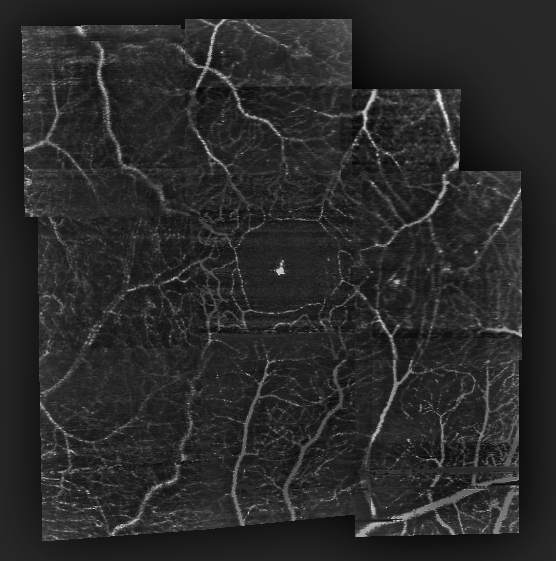
\includegraphics[width=10cm]{gfx/mosaic}
  \caption{Mozaika OCT stworzona z połączenia angiograficznych obrazów OCT.}
  \label{fig:algorytmy_korejestracji:mosaic}
\end{figure}

Proces automatycznego stworzenia mozaiki takiej jak na rysunku \ref{fig:algorytmy_korejestracji:mosaic} jest zadaniem nietrywialnym i wymaga dokładnej analizy wiedzy dziedzinowej oraz precyzyjnego wyboru metod. Pierwszym krokiem jest wybór modelu deformacji kafelków (sekcja \ref{sec:algorytmy_korejestracji:model_deformacji}), następnym etapem, który jest jednocześnie najbardziej wymagającym jest wybór metody wzajemnej korejestracji kafelków (sekcja \ref{sec:algorytmy_korejestracji:korejestracja_kafelow}). Posiadając zdefiniowane wzajemne relacje kafelków oraz ich docelowe położenie w finalnej mozaice należy wykonać proces łączenia kafelków (sekcja \ref{sec:algorytmy_korejestracji:laczenie_kafelkow}). W każdej z tych sekcji została wyjaśniona idea metody w kontekście stworzenia mozaiki OCT, natomiast szczegółowy opis zaimplementowanych metod znajduje się w rozdziale \ref{sec:proponowane_algorytmy}.

\section{Model deformacji kafelków}
\label{sec:algorytmy_korejestracji:model_deformacji}

Model deformacji kafelków określa dozwolone przekształcenia geometryczne, które odwzorują piksele kafelka do pikseli kafelka w finalnej mozaice. Ze względu na to, że angiograficzne obrazy OCT znajdują się na jednej płaszczyźnie możliwy zbiór modeli deformacji ogranicza nam się do transformacji dwuwymiarowych, które zostały zobrazowane na rysunku \ref{fig:algorytmy_korejestracji:trans}.

\begin{figure}[H]
  \centering
  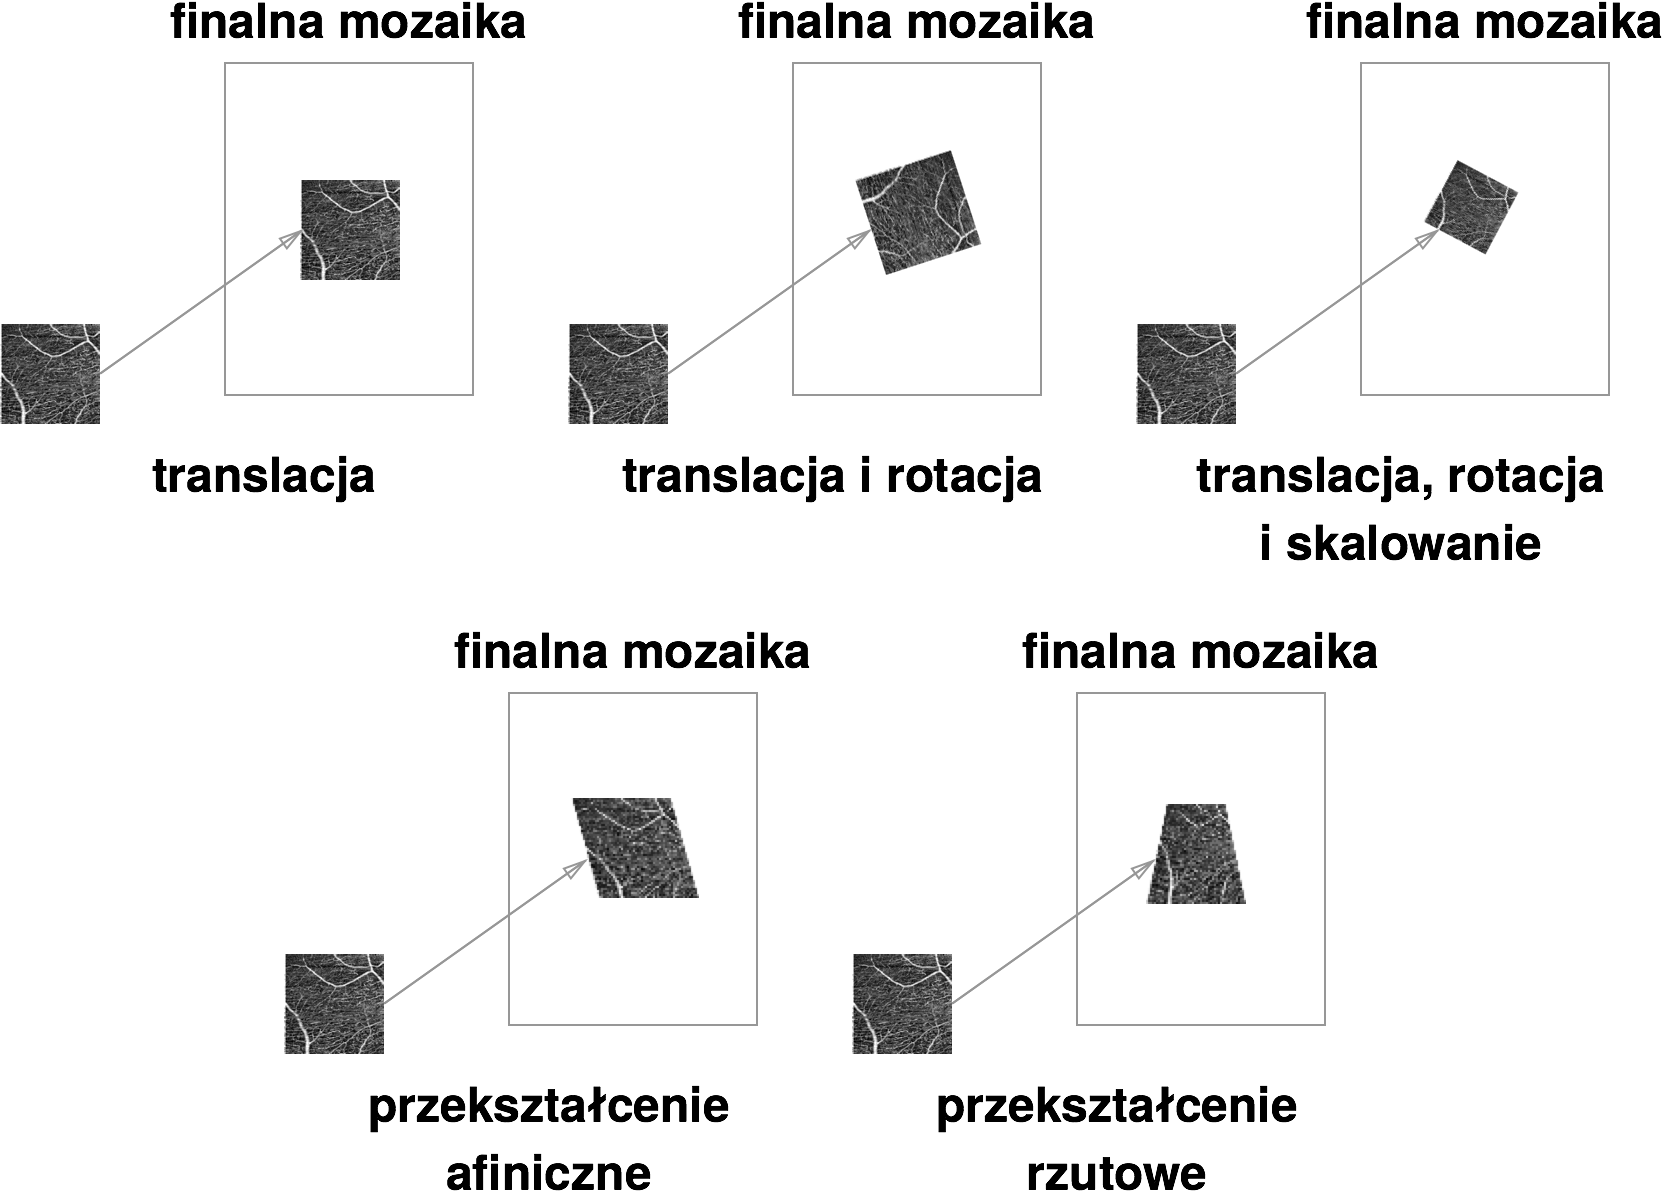
\includegraphics[width=\textwidth]{gfx/trans}
  \caption{Zbiór transformacji dwuwymiarowych dla przykładowego angiograficznego obrazu OCT.}
  \label{fig:algorytmy_korejestracji:trans}
\end{figure}

Idealnie OCT powinno tworzyć angiograficzne obrazy, które są względem siebie tylko przesunięte, natomiast w rzeczywistości pojawiają się zniekształcenia wynikające z niedokładności urządzenia oraz ruchu oka pacjenta, przez co niektóre kafelki są nieznacznie obrócone względem siebie. Z tego względu wybranym modelem deformacji kafelków został \textbf{model transformacji ciała sztywnego}, czyli połączenie translacji i rotacji.

\subsection{Matematyczny zapis modelu transformacji ciała sztywnego}

Współrzędne piksela w kafelku możemy określić jako trójelementowy wektor $\widetilde{x}=(x, y, 1)$, gdzie $x$ i $y$ to współrzędne piksela w układzie współrzędnych kafelka. Tak zdefiniowany piksel poddaje się transformacji by uzyskać współrzędne tego piksela $\hat{x}=(x', y')$ w układzie współrzędnych finalnej mozaiki. W sekcji \ref{sec:algorytmy_korejestracji:model_deformacji} została wybrana transformacja ciała sztywnego, który zakłada tylko translację oraz rotację i może być zapisana jako:

\begin{equation}
\hat{x}=\begin{bmatrix}R&t\end{bmatrix}\widetilde{x}
\label{eq:transformation}
\end{equation}

gdzie:

\begin{align}
R &= \begin{bmatrix}cos(\theta)&-sin(\theta)\\sin(\theta)&cos(\theta)\end{bmatrix} &&\text{i} & t &= \begin{bmatrix}t_{x}\\t_{y}\end{bmatrix}
\label{eq:rotation_and_translation}
\end{align}

W równaniu \ref{eq:rotation_and_translation} $\theta$ to kąt obrotu (rotacja) względem początku układu współrzędnych, a $t_{x}$ i $t_{y}$ to odpowiednio przesunięcia względem osi x i osi y. Parametry $\theta$, $t_{x}$ i $t_{y}$ są niewiadomymi równania \ref{eq:transformation}, których obliczenie jest tematem sekcji \ref{sec:algorytmy_korejestracji:korejestracja_kafelow}.

\section{Korejestracja kafelków}
\label{sec:algorytmy_korejestracji:korejestracja_kafelow}

Po wyborze modelu deformacji kafelków można przejść do wyboru metody, która będzie określać jego parametry (w przypadku niniejszej pracy są to parametry przesunięcia i obrotu). Metoda ta powinna zwrócić takie wartości by kafelek znalazł się w odpowiednim miejscu w finalnej mozaice z możliwie najmniejszym błędem. By rozwiązać ten problem najpierw trzeba poznać położenie kafelków względem siebie oraz ustalić kafelek referencyjny. Rysunek \ref{fig:algorytmy_korejestracji:reference_tile} przedstawia przykładowe rozmieszczenie kafelków. Kafelek referencyjny oznaczony poprzez przerywane linie jest przesuwany do finalnej mozaiki, natomiast żeby odpowiednio umieścić kafelki (2) i (3) trzeba najpierw znać dopasowanie kafelków (2) i (3) do kafelka referencyjnego (1). W przykładzie na rysunku \ref{fig:algorytmy_korejestracji:reference_tile} zostało założone, że kafelki (2) i (3) mogą być dopasowane do kafelka (1). Informacja na temat tego, które kafelki należy dopasować do których kafelek wynika z wiedzy dziedzinowej i opisane jest to w sekcji \ref{sec:proponowane_algorytmy:wiedza_dziedzinowa}.

\begin{figure}[H]
  \centering
  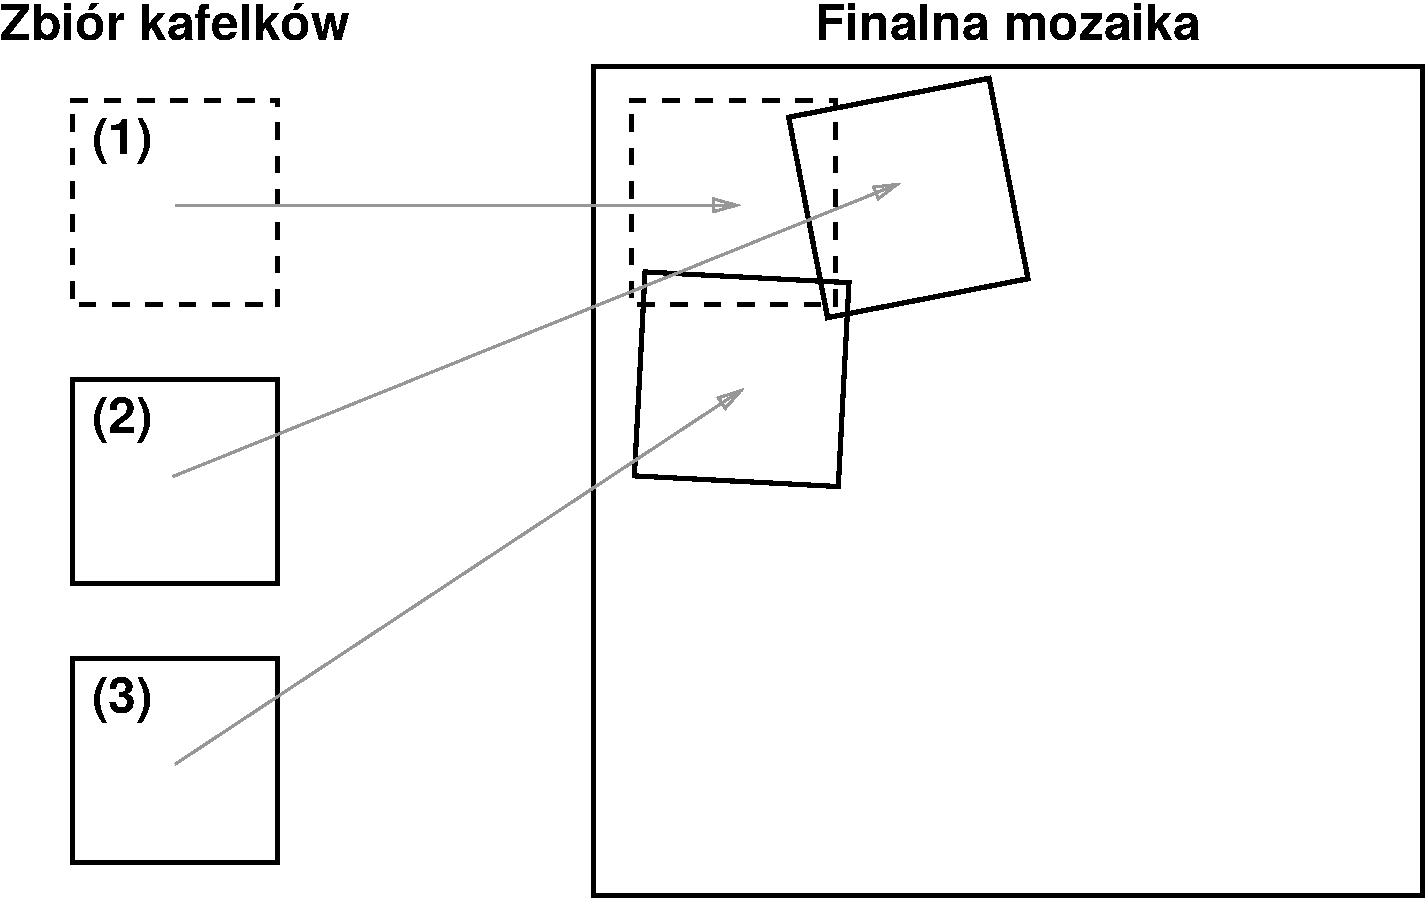
\includegraphics[width=\textwidth]{gfx/reference_tile}
  \caption{Przykładowe rozmieszczenie kafelków na finalnej mozaice. Kafelek referencyjny został wyróżniony przerywaną linią.}
  \label{fig:algorytmy_korejestracji:reference_tile}
\end{figure}

Dopasowanie dwóch kafelków do siebie nazywa się również ich korejestracją, czyli przeniesieniem dwóch kafelek do wspólnego układu współrzędnych w taki sposób by były względem siebie dopasowane. Prosty przykład korejestracji przedstawiony jest na rysunku \ref{fig:algorytmy_korejestracji:align}, gdzie dwie kafelki mają wspólny obszar nałożenia.

\begin{figure}[H]
  \centering
  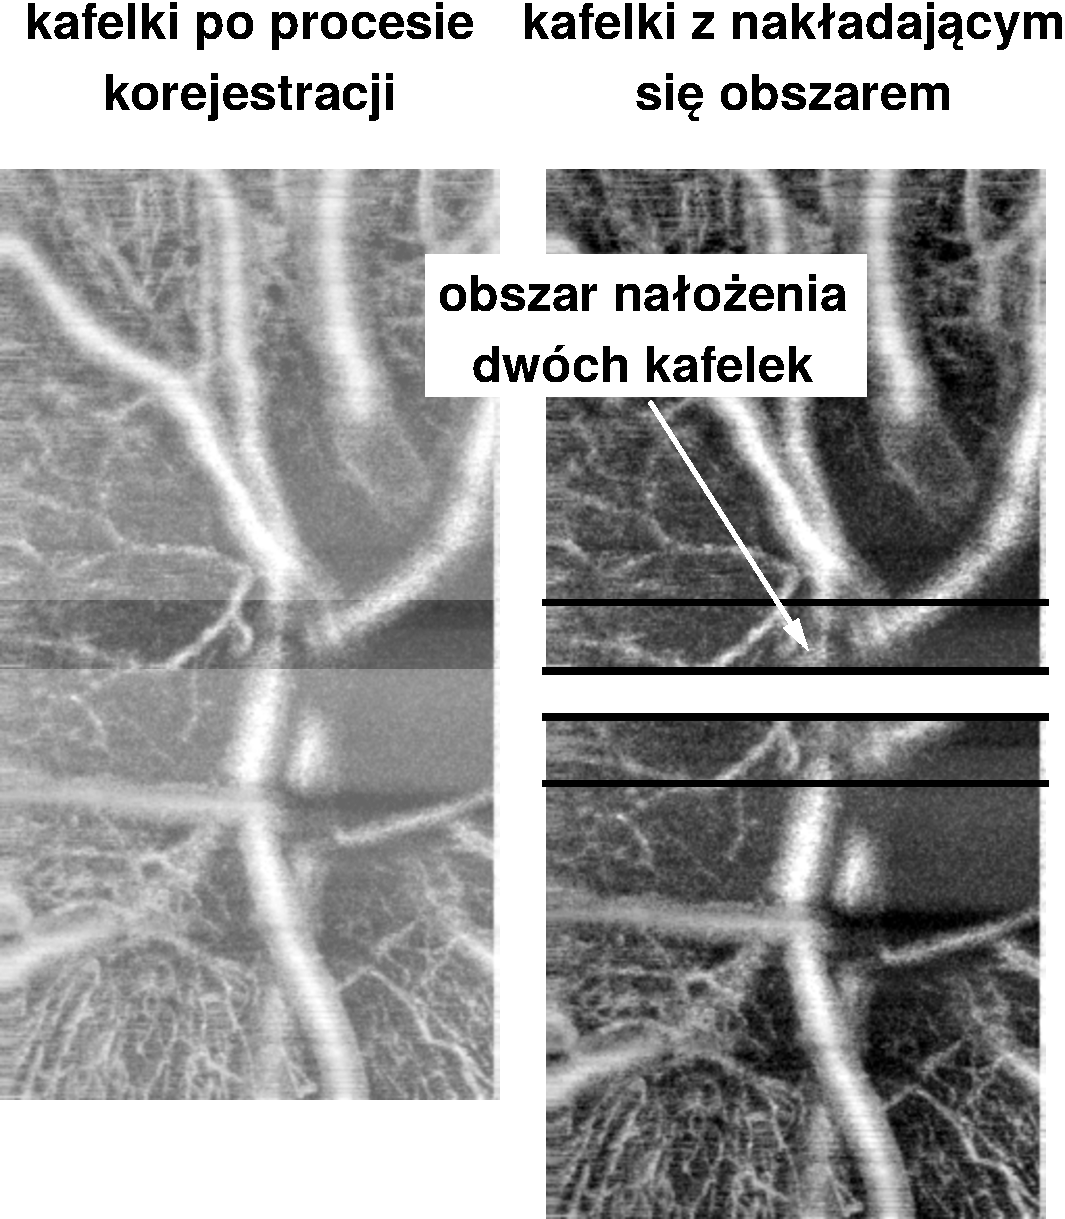
\includegraphics[width=7cm]{gfx/align}
  \caption{Przykładowa korejestracja dwóch kafelek ze wspólnym obszarem nałożenia.}
  \label{fig:algorytmy_korejestracji:align}
\end{figure}

Dopasowanie kafelków z rysunku \ref{fig:algorytmy_korejestracji:align} jest przykładem bardzo prostym, ponieważ wymaga tylko translacji jednej kafelki względem drugiej. W rzeczywistości pomiary OCT nie są tak dokładne przez co prosta translacja wzdłuż jednej z osi nie wystarcza i wymagane jest automatyczne wyznaczenie translacji wzdłuż z każdej z osi oraz parametru rotacji. Algorytmy korejestracji umożliwiające automatyczne dopasowanie można podzielić na dwie dziedziny:

\begin{enumerate}
\item Korejestracja na podstawie wartości pikseli (bezpośrednia).
\item Korejestracja na podstawie cech.
\end{enumerate}

\subsection{Korejestracja na podstawie wartości pikseli (bezpośrednie)}
\label{sec:algorytmy_korejestracji:korejestracja_na_podstawie_wartosci}

\subsection{Korejestracja na podstawie cech}
\label{sec:algorytmy_korejestracji:korejestracja_na_podstawie_cech}

\section{Łączenie kafelków}
\label{sec:algorytmy_korejestracji:laczenie_kafelkow}






















